%\Gls{ele} and \gls{photon} candidates can be reconstructed from detector outputs.
%The rare Higgs decay to \glspl{photon} is the simplest possible event signature to analyze.

%\textcolor{red}{\hrulefill \textsc{Unfinished SectionI}\hrulefill}\\
Now that the physical detectors have been described these individual physical detector read outs are translated into the representations of the physical particles that deposited the energy corresponding to those read outs. 
The four types of particles (electrons, photons, hadrons, muons) that can be directly detected at ATLAS are shown in Figure~\ref{fig:detector:objectreco}.
Particles which do not interact with the detector and escape ATLAS entirely can be inferred by imposing conservation of momentum in the $x$-$y$ plane.
As the initial state partons inside the proton have negligible momenta transverse to the proton beams, conservation of momentum implies that the sum of the momenta of the final state detected particles in the plane transverse to the proton beams should be zero, and any imbalance implies the presence of undetected particles like neutrinos.
\begin{figure}[h]
  \begin{center}
    \makebox[\textwidth][c]{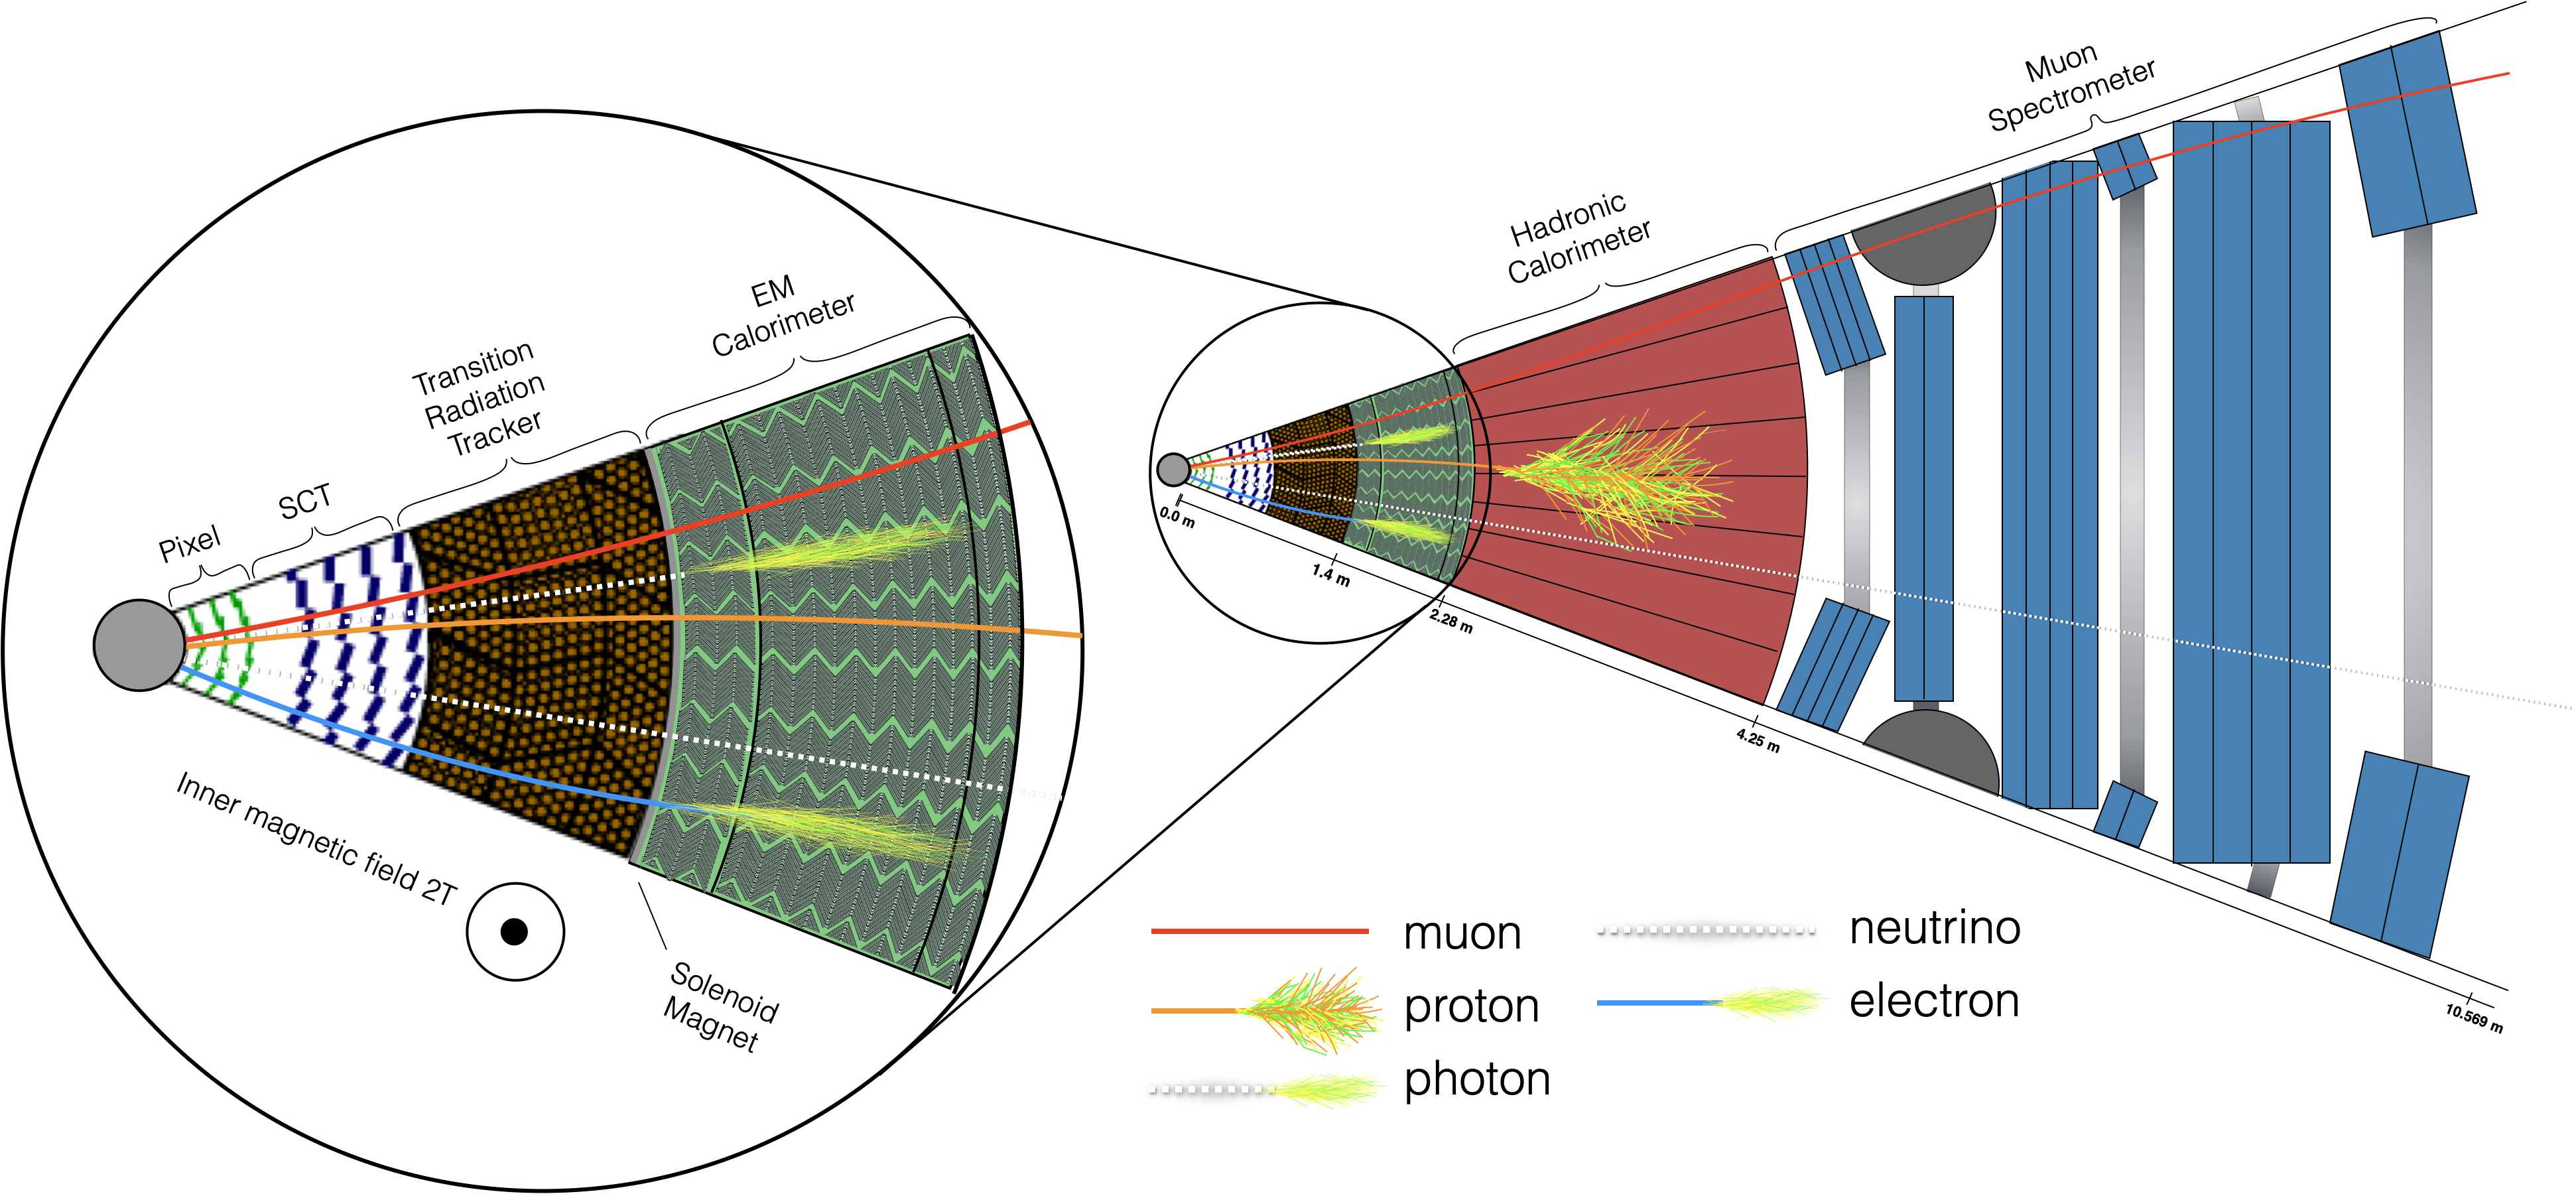
\includegraphics[width=1.25\textwidth]{figs/detector/ObjeRecoDefenseVersion.png}}
  \end{center}
  \caption[Particle signatures for different particle types when traversing the ATLAS detector.]
          {Particle signatures for different particle types when traversing the ATLAS detector in a radial direction.}
          \label{fig:detector:objectreco}
\end{figure}

\subsection{Electrons and Photons}
Electrons and photons are reconstructed from electromagnetic clusters deposited in the EM calorimeter layer.
The EM clusters that can then be matched to charged particle tracks are then reconstructed electrons, and those that can't, photons.
Further identification criteria are then used to distinguish electrons and photons from backgrounds.
A detailed discussion of electron identification is given in Chapter~\ref{ch:electronid}.

\subsection{Muons}
Muon reconstruction is first performed independently in the ID and MS. 
The information from individual subdetectors is then combined to form the muon tracks that are used in physics analyses~\cite{ATLAS:2016lqx}.
The combined reconstruction then proceeds in four different ways depending on the information available from each sub-detector~\cite{ATLAS:2016lqx}:
\begin{itemize}
    \item \emph{Combined (CB) muon}: track reconstruction is performed independently in the ID and MS, and a combined track is formed with a global refit that uses the hits from both the ID and MS sub-detectors.
    An outside-in algorithm where hits in the MS are extrapolated into the ID is the primary method with an inside-out algorithm acting as a complimentary approach.
    \item \emph{Segment-tagged (ST) muons}: a track in the ID is classified as a muon if, once extrapolated to the MS, it is associated with at least one local track segment in the MDT or cathode strip chambers (CSC).
    \item \emph{Calorimeter-tagged (CT) muons}: a track in the ID is identified as a muon if it can be matched to an energy deposit in the calorimeter compatible with a minimum-ionizing particle.
    \item \emph{Extrapolated (ME) muons}: the muon trajectory is reconstructed based only on the MS track and a loose requirement on compatibility with originating from the interaction point.
\end{itemize}
Overlaps between different muon types are resolved before producing the collection of muons used in physics analyses.
When two muon types share the same ID track, preference is given to CB muons, then to ST, and finally to CT muons. The overlap with ME muons in the muon system is resolved by analyzing the track hit content and selecting the track with better fit quality and larger number of hits\cite{ATLAS:2016lqx}.

\subsection{Hadrons and Jets}
%While isolated hadrons can be produced at the LHC via diffractive collisions the physics program at the LHC is primarily focused on physics produced via inelastic non-diffractive proton-proton collisions and for this thesis hadrons will only make an appearance in the detector as jets.
Jets were described from a theoretical stand point in Section~\ref{sec:theory:QCD}.
In ATLAS, jet reconstruction uses the energy clusters in the EM and hadronic calorimeters, as well as the reconstructed tracks from the ID from the charged particles in the jet.
Jet reconstruction can follow several recombination algorithms, however the most widely used algorithm at ATLAS is the anti-$kt$ algorithm ~\cite{Cacciari:2008gp, Cacciari:2011ma}.
At each step, the anti-kt algorithm combines the pair of objects that have the smallest distance apart, where the distance is measured as the angular separation ($\sqrt{\Delta \phi^2 + \Delta \eta^2}$) between the objects multiplied by the minimum of the inverse of the \et\ of either object.
Note that the weighting by the inverse \et\ gives rise to the ``anti-$kt$'' name and, more importantly,  means that the combination process starts with the highest \et\ cluster.
This combination process stops when the angular separation between objects exceeds a user-specified cone radius $R$, which is usually 0.4 for most ATLAS analyses.
The final combined object is called a jet. 

\subsection{Missing Transverse Energy}
The missing transverse energy serves as a proxy for particles that do not interact with any detector element.
In the $x$-$y$ plane, transverse to the proton beams, the missing transverse momentum points in the opposite direction to the total transverse momentum calculated from adding up the transverse momenta of the calibrated electrons, photons, muons, and jets, and any unclustered "soft" calorimeter deposits.
The missing transverse energy is the magnitude of the missing transverse momentum vector.